\subsection{\texorpdfstring{$y''-xy = 0$}{y''-xy = 0}}
Die bereits bekannte Airy-Differentialgleichung
\begin{align*}
	y''-xy = 0
\end{align*}
ergibt nun in die allgemeine L"osungsformel (\ref{eq:wellen:allgemeineloesung}) 
eingesetzt

\begin{equation*}
	\begin{split}
		y(x) &= a_0+a_1x-\sum_{k=2}^{\infty} \frac{1}{k(k-1)} ((-1) a_{k-2-1} + 
		0 
		a_{k-2-0}) x^k
		\\
		&= a_0+a_1x+\sum_{k=2}^{\infty} \frac{1}{k(k-1)} a_{k-3} x^k,
		\qquad a_{k < 0} = 0,
	\end{split}
\end{equation*}
was sich mit den bereits bekannten L"osung deckt.

Abbildung (\ref{fig:wellen:airy-dgl}) zeigt die genannten Konsequenzen deutlich 
auf.

\begin{figure}
	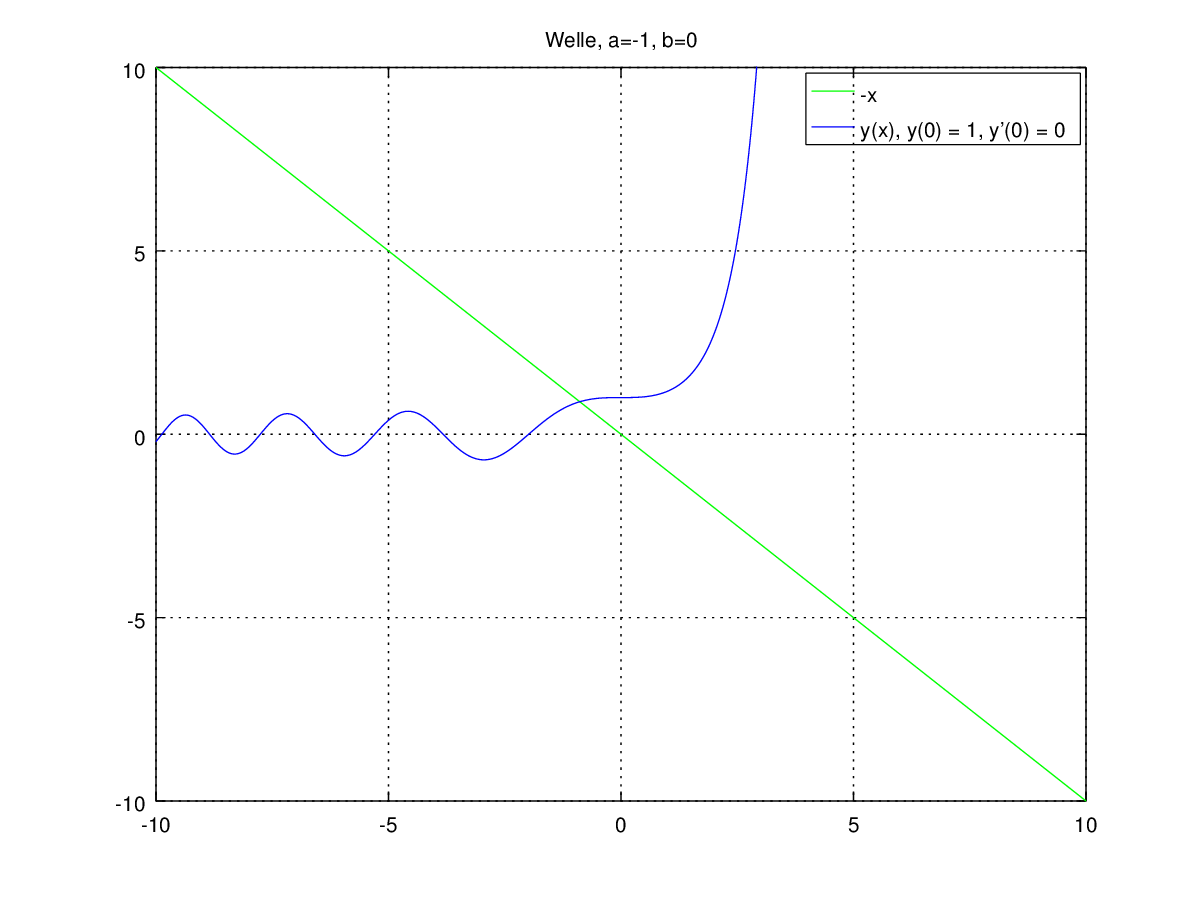
\includegraphics[scale=0.65]{./wellen/images/allgemein/n1.png}
	\caption{L"osung Airy-Differentialgleichung}
	\label{fig:wellen:airy-dgl}
\end{figure}